\documentclass{beamer}
\setbeamerfont{headline}{size=\footnotesize}

\mode<presentation>{
\usetheme{Montpellier}
\setbeamercovered{transparent}
\usecolortheme{lsc}
}

\mode<handout>{
  % tema simples para ser impresso
  \usepackage[bar]{beamerthemetree}
   % Colocando um fundo cinza quando for gerar transparências para serem impressas
  % mais de uma transparência por página
  \beamertemplatesolidbackgroundcolor{black!5}
}

\usepackage{fancyvrb}
\usepackage{pdfpages} % Pacote para incluir PDFs

\usepackage{amsmath,amssymb}
\usepackage[brazil]{varioref}
\usepackage[english,brazil]{babel}
\usepackage[utf8]{inputenc}
\usepackage{fontawesome}
\usepackage{ccicons}

\usepackage{makecell} % Adicione isso no preâmbulo do documento

%\usepackage[latin1]{inputenc}
\usepackage{graphicx}
\usepackage{listings}
\usepackage{url}
\usepackage{colortbl}
\usepackage{caption}
\usepackage{tikz}
\usepackage{transparent}
\usepackage{multirow}
\usepackage{graphicx}
\usepackage{listings}
\usepackage{exercise,chngcntr}

\usepackage{listings}
\usepackage{xcolor}
\usepackage{tikz}
\usetikzlibrary{shapes, arrows.meta, positioning}


% Definição de cores para o código Python
\definecolor{codegreen}{rgb}{0,0.6,0}
\definecolor{codegray}{rgb}{0.5,0.5,0.5}
\definecolor{codepurple}{rgb}{0.58,0,0.82}
\definecolor{backcolour}{rgb}{0.95,0.95,0.92}
% Configuração do estilo do código Python
\lstdefinestyle{mystyle}{
    xleftmargin=0pt,           % Aumenta a margem esquerda
    xrightmargin=10pt,          % Aumenta a margem direita
    frame=single,               % Adiciona um quadro ao redor do código
    framesep=10pt,              % Espaço entre o quadro e o código
    % Outras configurações do lstlisting...
    backgroundcolor=\color{backcolour},
    commentstyle=\color{codegreen},
    keywordstyle=\color{magenta},
    numberstyle=\tiny\color{codegray},
    stringstyle=\color{codepurple},
    basicstyle=\footnotesize\ttfamily,
    breakatwhitespace=false,
    breaklines=true,
    captionpos=b,
    keepspaces=true,
    %numbers=left,
    numbersep=5pt,
    showspaces=false,
    showstringspaces=false,
    showtabs=false,
    tabsize=2,
    basicstyle=\ttfamily, % Usa uma fonte de largura fixa para o código
    upquote=true,         % Tenta usar aspas retas se a fonte suportar,
    breakatwhitespace=false, % Quebra linhas em espaços em branco quando possível
}

\lstset{style=mystyle}


\beamertemplatetransparentcovereddynamic
\addtobeamertemplate{title page}{\centering{ 
\includegraphics[width=1.25cm]{figs/logo.png}}}{}
\title[]{Lógica Fuzzy}
\author[Elton Sarmanho]{ 
Professor: Elton Sarmanho\inst{1} 
\newline
E-mail: \href{mailto:eltonss@ufpa.br}{eltonss@ufpa.br}\newline
\href{https://github.com/eltonsarmanho}{\faGithub} \href{https://www.linkedin.com/in/elton-sarmanho-836553185/}{\faLinkedinSquare}\\
\ccbyncsa
}   
  \institute[UFPA]{
   \inst{1}%
     Faculdade de Sistemas de Informação - UFPA/CUNTINS
     }     
 
% Se comentar a linha abaixo, irá aparecer a data quando foi compilada a apresentação  
\date{\today}
\pgfdeclareimage[height= 1.25 cm]{inf}{figs/logo.png}
% pode-se colocar o LOGO assim
\logo{{\transparent{0.35}\pgfuseimage{inf}}}

% \AtBeginSection[]{
%   \begin{frame}<beamer>
%     \frametitle{Roteiro}
%     \tableofcontents[currentsection,currentsubsection]
%   \end{frame}  
% }

\setbeamertemplate{navigation symbols}{\insertframenavigationsymbol \insertsectionnavigationsymbol \insertbackfindforwardnavigationsymbol} 


\expandafter\def\expandafter\insertshorttitle\expandafter{%
  \insertshorttitle\hfill%
  \insertframenumber\,/\,\inserttotalframenumber}
  \renewcounter{Exercise}[section]
  \newcounter{Example}



\begin{document}

\setbeamertemplate{logo}{}
\begin{frame}
\titlepage
\end{frame}
%Começar mostrar Logo apos slide de titulo
\logo{{\transparent{0.35}\pgfuseimage{inf}}}

\begin{frame}
\frametitle{Roteiro}
\tableofcontents[sections={1-3}]
\end{frame}
\begin{frame}
\frametitle{Roteiro}
\tableofcontents[sections={4-6}]
\end{frame}

\begin{frame}
\frametitle{Roteiro}
\tableofcontents[sections={7-8}]
\end{frame}
\begin{frame}{Licença}
    Este trabalho está licenciado sob a licença Creative Commons:

    \bigskip
    \ccbyncsa
\end{frame}
%Declaração das Imagens da Apresentação

%%%%%%%%%%%%%%%%%%%%%%%%%%%%%%%%%%%%%%%%
\section{Planejamento}

\begin{frame}
Nesta aula:

\begin{itemize}
 \item Vamos explorar os conceitos fundamentais de lógica fuzzy.
 \item Ter panorama sobre conceito.
 \item Códigos do Professor estão no github
\end{itemize}


\end{frame}

\section{Fundamentação}
\subsection{Conceitos Fundamentais}
\begin{frame}
\centering
\Huge
\textbf{Conceitos\\Fundamentais}
\end{frame}

\begin{frame}{O que é Lógica Fuzzy?}
    \begin{itemize}
        \item A lógica fuzzy (ou lógica difusa) é uma extensão da lógica clássica que permite graus de pertinência entre 0 e 1.
        \item Ela é ideal para lidar com incertezas e informações imprecisas.
    \end{itemize}
    \pause
    \begin{block}{Definição Formal}
        \textbf{Conjunto fuzzy}: Um conjunto \( A \) em um universo \( X \) é caracterizado por uma função de pertinência \( \mu_A: X \to [0, 1] \), onde:
        \begin{itemize}
            \item \( \mu_A(x) = 1 \): Totalmente pertencente ao conjunto \( A \).
            \item \( \mu_A(x) = 0 \): Não pertencente ao conjunto \( A \).
            \item \( 0 < \mu_A(x) < 1 \): Pertinência parcial.
        \end{itemize}
    \end{block}
\end{frame}

\begin{frame}{Comparação: Lógica Clássica vs. Lógica Fuzzy}
    \centering
    \begin{tikzpicture}
        % Eixos
        \draw[->] (0, 0) -- (6, 0) node[right] {$x$};
        \draw[->] (0, 0) -- (0, 3) node[above] {$\mu(x)$};

        % Lógica Clássica
        \draw[thick] (0, 0) -- (2, 0) -- (2, 2) -- (4, 2) -- (4, 0) -- (6, 0);
        \node[below] at (3, 0) {\footnotesize Lógica Clássica};

        % Lógica Fuzzy
        \draw[thick, smooth, blue] (0, 0) .. controls (2, 0.5) and (4, 1.5) .. (6, 2);
        \node[above] at (3, 1.5) {\footnotesize Lógica Fuzzy};
    \end{tikzpicture}
    \vspace{0.5cm}
    \begin{itemize}
        \item \textbf{Lógica Clássica:} Valores discretos (0 ou 1).
        \item \textbf{Lógica Fuzzy:} Valores contínuos entre 0 e 1.
    \end{itemize}
\end{frame}

\begin{frame}{Exemplo Gráfico de Conjunto Fuzzy}
    \centering
    \begin{tikzpicture}
        \draw[->] (0, 0) -- (5, 0) node[right] {$x$};
        \draw[->] (0, 0) -- (0, 3) node[above] {$\mu_A(x)$};

        \draw[thick, blue, domain=0:4] plot[smooth] (\x, {2*\x/4}) node[above right] {\footnotesize Crescente};
        \draw[thick, red, domain=4:5] plot[smooth] (\x, {2*(5-\x)}) node[above right] {\footnotesize Decrescente};

        \draw[dashed] (4, 0) -- (4, 3) node[above right] {\footnotesize Pico};
    \end{tikzpicture}
    \vspace{0.5cm}
    \begin{itemize}
        \item A função de pertinência \( \mu_A(x) \) representa o grau de pertencimento do elemento \( x \) ao conjunto fuzzy \( A \).
    \end{itemize}
\end{frame}

\begin{frame}{Função de Pertinência}
    \begin{block}{Definição}
        A função de pertinência \( \mu_A(x) \) de um conjunto fuzzy \( A \) mapeia cada elemento \( x \in X \) em um valor no intervalo \([0, 1]\), representando o grau de pertencimento de \( x \) ao conjunto \( A \).
    \end{block}
    \pause
    \begin{itemize}
        \item \textbf{Exemplo de funções comuns:}
        \begin{itemize}
            \item \textbf{Triangular:} \( \mu_A(x) = \max\left(0, \min\left(\frac{x-a}{b-a}, \frac{c-x}{c-b}\right)\right) \)
            \item \textbf{Trapezoidal:} \( \mu_A(x) = \max\left(0, \min\left(\frac{x-a}{b-a}, 1, \frac{d-x}{d-c}\right)\right) \)
            \item \textbf{Gaussiana:} \( \mu_A(x) = e^{-\frac{(x-c)^2}{2\sigma^2}} \)
        \end{itemize}
    \end{itemize}

\end{frame}

\begin{frame}{Função de Pertinência}
    \centering
 \begin{figure}[h]
         \centering
         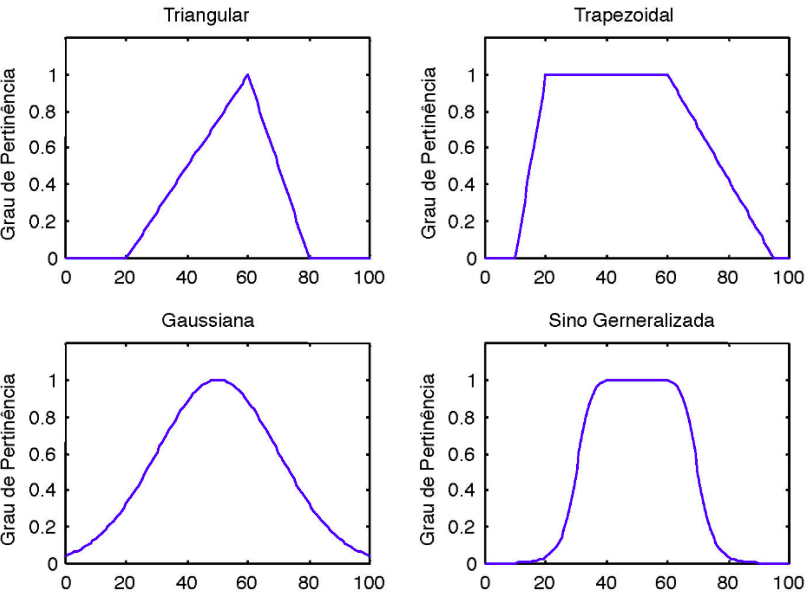
\includegraphics[width=0.9\textwidth]{figs/funcao.png}
    \end{figure}
\end{frame}



\begin{frame}{Variáveis Linguísticas}
\footnotesize
    \begin{block}{}
        \textbf{Definição}: uma variável linguística é uma variável cujo valor não é um número, mas sim uma palavra ou sentença em linguagem natural.
    \end{block}
    \pause
    \begin{itemize}
        \item \textbf{Exemplo:} Velocidade de um carro
        \begin{itemize}
            \item Valores possíveis: \textit{lento}, \textit{moderado}, \textit{rápido}
        \end{itemize}
        \item Cada valor linguístico é associado a um conjunto fuzzy.
    \end{itemize}
    \pause
    \centering
    \begin{tikzpicture}
        % Eixos
        \draw[->] (0, 0) -- (6, 0) node[right] {Velocidade};
        \draw[->] (0, 0) -- (0, 3) node[above] {Grau de Pertinência};

        % Conjuntos fuzzy
        \draw[thick, blue] (0, 0) -- (2, 2) -- (4, 0) node[below] {\footnotesize Lento};
        \draw[thick, red] (2, 0) -- (4, 2) -- (6, 0) node[below] {\footnotesize Moderado};
        \draw[thick, green] (4, 0) -- (6, 2) -- (8, 0) node[below] {\footnotesize Rápido};
    \end{tikzpicture}
\end{frame}

\begin{frame}{Operações Básicas em Conjuntos Fuzzy}
\footnotesize
    \begin{block}{Operações Fundamentais}
        \begin{itemize}
            \item \textbf{Interseção (AND):} \( \mu_{A \cap B}(x) = \min(\mu_A(x), \mu_B(x)) \)
            \item \textbf{União (OR):} \( \mu_{A \cup B}(x) = \max(\mu_A(x), \mu_B(x)) \)
            \item \textbf{Complemento (NOT):} \( \mu_{\neg A}(x) = 1 - \mu_A(x) \)
        \end{itemize}
    \end{block}
    \centering
    \begin{tikzpicture}
        % Eixos
        \draw[->] (0, 0) -- (6, 0) node[right] {$x$};
        \draw[->] (0, 0) -- (0, 3) node[above] {$\mu(x)$};

        % Conjunto A
        \draw[thick, blue] (0, 0) -- (2, 2) -- (4, 0) node[below] {\footnotesize A};

        % Conjunto B
        \draw[thick, red] (1, 0) -- (3, 2) -- (5, 0) node[below] {\footnotesize B};


    \end{tikzpicture}
\end{frame}



\begin{frame}{Operações Básicas em Conjuntos Fuzzy}
\footnotesize
    \begin{block}{Operações Fundamentais}
        \begin{itemize}
            \item \textbf{Interseção (AND):} \( \mu_{A \cap B}(x) = \min(\mu_A(x), \mu_B(x)) \)
            \item \textbf{União (OR):} \( \mu_{A \cup B}(x) = \max(\mu_A(x), \mu_B(x)) \)
            \item \textbf{Complemento (NOT):} \( \mu_{\neg A}(x) = 1 - \mu_A(x) \)
        \end{itemize}
    \end{block}
    \centering
    \begin{tikzpicture}
        % Eixos
        \draw[->] (0, 0) -- (6, 0) node[right] {$x$};
        \draw[->] (0, 0) -- (0, 3) node[above] {$\mu(x)$};

        % Conjunto A
        \draw[thick, blue,opacity=0.1] (0, 0) -- (2, 2) -- (4, 0) node[below] {\footnotesize A};

        % Conjunto B
        \draw[thick, red,opacity=0.1] (1, 0) -- (3, 2) -- (5, 0) node[below] {\footnotesize B};

        % Interseção
        \draw[thick, purple, densely dashed] (1., 0) -- (2.5, 1.5) -- (4, 0) node[below] {\footnotesize $A \cap B$};

    \end{tikzpicture}
\end{frame}


\begin{frame}{Operações Básicas em Conjuntos Fuzzy}
\footnotesize
    \begin{block}{Operações Fundamentais}
        \begin{itemize}
            \item \textbf{Interseção (AND):} \( \mu_{A \cap B}(x) = \min(\mu_A(x), \mu_B(x)) \)
            \item \textbf{União (OR):} \( \mu_{A \cup B}(x) = \max(\mu_A(x), \mu_B(x)) \)
            \item \textbf{Complemento (NOT):} \( \mu_{\neg A}(x) = 1 - \mu_A(x) \)
        \end{itemize}
    \end{block}
    \centering
    \begin{tikzpicture}
        % Eixos
        \draw[->] (0, 0) -- (6, 0) node[right] {$x$};
        \draw[->] (0, 0) -- (0, 3) node[above] {$\mu(x)$};

          % União
        \draw[thick, orange, dotted] (0, 0) -- (2, 2) -- (3, 2) -- (5, 0) node[below] {\footnotesize $A \cup B$};

        % Conjunto A
        \draw[thick, blue,opacity=0.1] (0, 0) -- (2, 2) -- (4, 0) node[below] {\footnotesize A};

        % Conjunto B
        \draw[thick, red,opacity=0.1] (1, 0) -- (3, 2) -- (5, 0) node[below] {\footnotesize B};



    \end{tikzpicture}
\end{frame}


\begin{frame}{Operações Básicas em Conjuntos Fuzzy}
\footnotesize
    \begin{block}{Operações Fundamentais}
        \begin{itemize}
            \item \textbf{Interseção (AND):} \( \mu_{A \cap B}(x) = \min(\mu_A(x), \mu_B(x)) \)
            \item \textbf{União (OR):} \( \mu_{A \cup B}(x) = \max(\mu_A(x), \mu_B(x)) \)
            \item \textbf{Complemento (NOT):} \( \mu_{\neg A}(x) = 1 - \mu_A(x) \)
        \end{itemize}
    \end{block}
    \centering
    \begin{tikzpicture}
        % Eixos
        \draw[->] (0, 0) -- (6, 0) node[right] {$x$};
        \draw[->] (0, 0) -- (0, 3) node[above] {$\mu(x)$};

        % Conjunto A
        \draw[thick, blue,opacity=0.2] (0, 0) -- (2, 2) -- (4, 0) node[below] {\footnotesize A};

        % Conjunto B
        \draw[thick, red,opacity=0.2] (1, 0) -- (3, 2) -- (5, 0) node[below] {\footnotesize B};


        % Complemento de A
        \draw[thick, green, dash dot] (0, 2) -- (2, 0) -- (4, 2) node[below] {\footnotesize $\neg A$};
    \end{tikzpicture}
\end{frame}

\begin{frame}{Normas e Conormas (T-norms e T-conorms)}
\footnotesize
    \begin{block}{Definição}
        \begin{itemize}
            \item \textbf{T-norms (Normas triangulares):} Modelam a operação de conjunção (AND) em lógica fuzzy.
            \item \textbf{T-conorms (Conormas triangulares):} Modelam a operação de disjunção (OR) em lógica fuzzy.
        \end{itemize}
    \end{block}
    \pause
    \begin{block}{Propriedades}
        \begin{itemize}
            \item \textbf{T-norm:} Monotonicidade, comutatividade, associatividade, identidade em 1.
            \item \textbf{T-conorm:} Monotonicidade, comutatividade, associatividade, identidade em 0.
        \end{itemize}
    \end{block}
    \pause
    \centering
    \begin{itemize}
        \item \textbf{Exemplo de T-norm:} \( \min(\mu_A(x), \mu_B(x)) \)
        \item \textbf{Exemplo de T-conorm:} \( \max(\mu_A(x), \mu_B(x)) \)
    \end{itemize}
\end{frame}

\begin{frame}{Questão}
\footnotesize
Considere os seguintes subconjuntos fuzzy \( A(x) \) e \( B(x) \):

\[
A(x) =
\begin{cases}
x & \text{se } x \in [0, 1], \\
-x + 3 & \text{se } x \in [1, 3], \\
0 & \text{caso contrário}.
\end{cases}
\]

\[
B(x) =
\begin{cases}
2x & \text{se } x \in [0, 1], \\
1 & \text{se } x \in [1, 2], \\
-2x + 6 & \text{se } x \in [2, 3], \\
0 & \text{caso contrário}.
\end{cases}
\]

\textbf{Questão:}
\begin{enumerate}
    \item Calcule a interseção fuzzy \( A(x) \cap B(x) \) usando \( \mu_{A \cap B}(x) = \min(A(x), B(x)) \).
    \item Esboce o gráfico da interseção \( A(x) \cap B(x) \).
\end{enumerate}
\end{frame}

\begin{frame}{Dicas para Resolução}
\textbf{Passos para resolver:}
\begin{itemize}
    \item Identifique os intervalos em que \( A(x) \) e \( B(x) \) estão definidos.
    \item Para cada intervalo, calcule \( \min(A(x), B(x)) \).
    \item Combine os resultados para formar a função \( A(x) \cap B(x) \).
    \item Esboce o gráfico final.
\end{itemize}
\end{frame}

\begin{frame}{Passo 1: Identificação dos Intervalos}
\textbf{Intervalos relevantes:}
\begin{itemize}
    \item \( x \in [0, 1]: \)
    \[
    A(x) = x, \quad B(x) = 2x.
    \]
    \item \( x \in [1, 2]: \)
    \[
    A(x) = -x + 3, \quad B(x) = 1.
    \]
    \item \( x \in [2, 3]: \)
    \[
    A(x) = -x + 3, \quad B(x) = -2x + 6.
    \]
\end{itemize}

\textbf{Fórmula da interseção:}
\[
\mu_{A \cap B}(x) = \min(A(x), B(x)).
\]
\end{frame}

\begin{frame}{Passo 2: Cálculo em Cada Intervalo}
\footnotesize
\textbf{Cálculos:}
\begin{itemize}
    \item Para \( x \in [0, 1]: \)
    \[
    A(x) = x, \quad B(x) = 2x.
    \]
    \[
    \mu_{A \cap B}(x) = \min(x, 2x) = x, \text{ pois } x \leq 2x \text{ nesse intervalo}.
    \]

    \item Para \( x \in [1, 2]: \)
    \[
    A(x) = -x + 3, \quad B(x) = 1.
    \]
    \[
    \mu_{A \cap B}(x) = \min(-x + 3, 1).
    \]

    \item Para \( x \in [2, 3]: \)
    \[
    A(x) = -x + 3, \quad B(x) = -2x + 6.
    \]
    \[
    \mu_{A \cap B}(x) = \min(-x + 3, -2x + 6).
    \]
\end{itemize}
\end{frame}

\begin{frame}{Passo 3: Resultados da Interseção}
\textbf{Função resultante:}
\[
\mu_{A \cap B}(x) =
\begin{cases}
x & \text{se } x \in [0, 1], \\
\min(-x + 3, 1) & \text{se } x \in [1, 2], \\
\min(-x + 3, -2x + 6) & \text{se } x \in [2, 3], \\
0 & \text{caso contrário}.
\end{cases}
\]

\textbf{Simplificando:}
\begin{itemize}
    \item Para \( x \in [0, 1]: \) \( \mu_{A \cap B}(x) = x \).
    \item Para \( x \in [1, 2]: \) \( \mu_{A \cap B}(x) = -x + 3 \) (pois \( -x + 3 \leq 1 \)).
    \item Para \( x \in [2, 3]: \) \( \mu_{A \cap B}(x) = -x + 3 \) (pois \( -x + 3 \leq -2x + 6 \)).
\end{itemize}
\end{frame}



\begin{frame}{Gráfico da Interseção \(A(x) \cap B(x)\)}
\begin{center}
\begin{tikzpicture}[scale=2]
    % Eixos
    \draw[->] (-0.5,0) -- (3.5,0) node[right] {\(x\)};
    \draw[->] (0,-0.5) -- (0,1.5) node[above] {\(\mu(x)\)};

    % Interseção A(x) ∩ B(x)
    \draw[green, thick] (0,0) -- (1,1) -- (2,1) -- (3,0) node[right] {\(A(x) \cap B(x)\)};
\end{tikzpicture}
\end{center}
\end{frame}


\begin{frame}{Gráfico dos Conjuntos Fuzzy}
\textbf{Gráfico de \( A(x) \) e \( B(x) \):}
\begin{center}
\begin{tikzpicture}[scale=2]
    % Eixos para A(x)
    \draw[->] (-0.5,0) -- (3.5,0) node[right] {\(x\)};
    \draw[->] (0,-0.5) -- (0,2.5) node[above] {\(\mu(x)\)};

    % Conjunto A(x)
    \draw[blue, thick] (0,0) -- (1,1) -- (3,0) node[right] {\(A(x)\)};

    % Conjunto B(x)
    \draw[red, thick] (0,0) -- (1,2) -- (2,1) -- (3,0) node[right] {\(B(x)\)};
\end{tikzpicture}
\end{center}
\end{frame}

\begin{frame}{Gráfico da Interseção}
\textbf{Gráfico da função \( \mu_{A \cap B}(x) \):}
\begin{center}
\begin{tikzpicture}[scale=2]
    % Eixos
    \draw[->] (-0.5,0) -- (3.5,0) node[right] {\(x\)};
    \draw[->] (0,-0.5) -- (0,1.5) node[above] {\(\mu(x)\)};

    % A(x)
    \draw[blue, thick,opacity=0.2] (0,0) -- (1,1) -- (3,0) node[right] {\(A(x)\)};

    % B(x)
    \draw[red, thick,opacity=0.2] (0,0) -- (1,2) -- (2,1) -- (3,0) node[right] {\(B(x)\)};

    % Interseção
    \draw[green, thick] (0,0) -- (1,1) -- (2,1) -- (3,0) node[right] {\(A(x) \cap B(x)\)};
\end{tikzpicture}
\end{center}
\end{frame}

\section{Inferência Fuzzy}
\begin{frame}
\centering
\Huge
\textbf{Inferência\\Fuzzy}
\end{frame}
\subsection{Regras Fuzzy}
\footnotesize
\begin{frame}{Inferência Fuzzy e Regras Fuzzy}
    \begin{block}{Inferência Fuzzy}
        O processo de inferência fuzzy é usado para derivar conclusões a partir de regras fuzzy aplicadas a dados de entrada imprecisos ou incertos.
    \end{block}
    \pause
    \begin{block}{Regras Fuzzy}
        Regras fuzzy são declaradas na forma de sentenças condicionais:
        \begin{itemize}
            \item \textbf{Forma geral:} \textit{SE} antecedente \textit{ENTÃO} consequente
            \item \textbf{Exemplo:} \textit{SE temperatura é alta ENTÃO velocidade do ventilador é alta}
        \end{itemize}
    \end{block}
    \pause
    \begin{itemize}
        \item Regras fuzzy utilizam variáveis linguísticas e suas funções de pertinência para determinar resultados.
        \item A agregação de regras permite combinar múltiplas condições.
    \end{itemize}
    \pause
    \centering
    \begin{tikzpicture}
        % Fluxo da inferência fuzzy
        \node[draw, rectangle, rounded corners, align=center] (input) at (0, 0) {Entradas Fuzzy};
        \node[draw, rectangle, rounded corners, align=center, right=of input] (rules) {Base de Regras Fuzzy};
        \node[draw, rectangle, rounded corners, align=center, right=of rules] (output) {Saídas Fuzzy};

        \draw[->] (input) -- (rules);
        \draw[->] (rules) -- (output);
    \end{tikzpicture}
\end{frame}
\subsection{Sistemas de Inferência Fuzzy}
\begin{frame}{Sistemas de Inferência Fuzzy}
    \begin{block}{Método de Mamdani}

        \begin{itemize}
            \item Um dos métodos mais usados para inferência fuzzy.
            \item As saídas fuzzy são obtidas por um processo de agregação e defuzzificação.
            \item Adequado para sistemas onde as regras são interpretáveis e compreensíveis.
        \end{itemize}
    \end{block}
    \begin{block}{Exemplo de Regras de Mamdani}
        \begin{itemize}
            \item SE temperatura é alta ENTÃO ventilador é rápido.
            \item SE temperatura é baixa ENTÃO ventilador é lento.
        \end{itemize}
    \end{block}
\end{frame}

\begin{frame}{Método de Sugeno}
    \begin{block}{Características principais}

        \begin{itemize}
            \item Baseado em expressões matemáticas ou funções lineares.
            \item A saída fuzzy é convertida diretamente em um valor numérico, sem defuzzificação.
            \item Adequado para sistemas complexos e onde é necessário controle preditivo.
        \end{itemize}
    \end{block}
    \begin{block}{Exemplo de Regras de Sugeno}
        \begin{itemize}
            \item SE temperatura é alta ENTÃO velocidade = 5 + 2\(temp\)
            \item SE temperatura é baixa ENTÃO velocidade = 1 + 0.5\(temp\)
        \end{itemize}
    \end{block}
\end{frame}

\begin{frame}{Comparação entre Mamdani e Sugeno}
    \begin{block}{Diferenças principais}
        \begin{itemize}
            \item \textbf{Mamdani:}
                \begin{itemize}
                    \item Foco em interpretabilidade.
                    \item Saída é uma função fuzzy que requer defuzzificação.
                \end{itemize}
            \item \textbf{Sugeno:}
                \begin{itemize}
                    \item Foco em precisão e simplicidade computacional.
                    \item Saída é numérica, sem necessidade de defuzzificação.
                \end{itemize}
        \end{itemize}
    \end{block}
    \begin{block}{Aplicações}
        \begin{itemize}
            \item \textbf{Mamdani:} Sistemas de suporte à decisão, controle de dispositivos como ventiladores e condicionadores de ar.
            \item \textbf{Sugeno:} Controle avançado de sistemas complexos, como robótica e automação industrial.
        \end{itemize}
    \end{block}
\end{frame}

\subsection{Agregação e Defuzzificação}
\footnotesize
\begin{frame}{}
    \begin{block}{Agregação}
        \begin{itemize}
            \item Combina as saídas fuzzy de todas as regras aplicáveis para formar um único conjunto fuzzy.
            \item Métodos comuns de agregação:
            \begin{itemize}
                \item União: \( \mu_{agregado}(x) = \max(\mu_{regra1}(x), \mu_{regra2}(x), \ldots) \)
                \item Soma: \( \mu_{agregado}(x) = \sum \mu_{regra_i}(x) \)
            \end{itemize}
        \end{itemize}
    \end{block}
    \pause
    \begin{block}{Defuzzificação}
        \begin{itemize}
            \item Converte o conjunto fuzzy agregado em um valor numérico para uso no mundo real.
            \item Métodos comuns de defuzzificação:
            \begin{itemize}
                \item Centro de Gravidade (CoG): \( y = \frac{\int x \cdot \mu(x) dx}{\int \mu(x) dx} \)
                \item Média dos Máximos (MoM): \( y = \text{média}(x \text{ onde } \mu(x) \text{ é máximo}) \)
                \item Altura: \( y = \sum \mu(x_i) \cdot x_i / \sum \mu(x_i) \)
            \end{itemize}
        \end{itemize}
    \end{block}
\end{frame}
\section{Sistemas de Controle Fuzzy}
\begin{frame}
\centering
\Huge
\textbf{Sistemas\\de\\Controle Fuzzy}
\end{frame}
\subsection{Controladores Fuzzy}

\begin{frame}{Controladores Fuzzy}

    \begin{block}{Definição}
        Um controlador fuzzy é um sistema que utiliza lógica fuzzy para determinar as ações de controle baseadas em entradas incertas ou imprecisas.
    \end{block}

\end{frame}

\begin{frame}{Componentes de um Controlador Fuzzy}
    \begin{itemize}
            \item \textbf{Fuzzificação:}
            \begin{itemize}
                \item Transforma as entradas nítidas (crisp) em valores fuzzy.
                \item Usa funções de pertinência para determinar o grau de pertencimento das entradas aos conjuntos fuzzy definidos.
            \end{itemize}
            \item \textbf{Inferência:}
            \begin{itemize}
                \item Aplica regras fuzzy para avaliar as condições e determinar as saídas fuzzy correspondentes.
                \item Utiliza operadores lógicos fuzzy (e.g., AND, OR) para combinar as regras.
            \end{itemize}

        \end{itemize}
 \end{frame}

 \begin{frame}{Componentes de um Controlador Fuzzy}
    \begin{itemize}
            \item \textbf{Defuzzificação:}
            \begin{itemize}
                \item Converte as saídas fuzzy em um valor nítido (crisp) para aplicação no sistema controlado.
                \item Métodos comuns incluem:
                \begin{itemize}
                    \item Centro de Gravidade (CoG): Proporciona equilíbrio considerando toda a área do conjunto fuzzy agregado.
                    \item Média dos Máximos (MoM): Usa o valor médio dos pontos com grau de pertinência máximo.
                \end{itemize}
            \end{itemize}
        \end{itemize}
 \end{frame}

\begin{frame}{Componentes de um Controlador Fuzzy}
    \begin{block}{Exemplo de Aplicação}
        \begin{itemize}
            \item Controle de temperatura: SE temperatura é alta ENTÃO potência do ar-condicionado é alta.
            \item Controle de velocidade: SE distância do carro da frente é pequena ENTÃO velocidade é baixa.
        \end{itemize}
    \end{block}
\end{frame}

\section{Python para Lógica Fuzzy}
\begin{frame}
\centering
\Huge
\textbf{Python\\para\\Lógica Fuzzy}
\end{frame}
\begin{frame}{}
    \begin{block}{Por que Python?}
        \begin{itemize}
            \item Python é uma linguagem amplamente usada em ciência de dados e inteligência artificial.
            \item Oferece bibliotecas especializadas para lógica fuzzy, como o \texttt{scikit-fuzzy}.
            \item Possui uma sintaxe simples, ideal para prototipagem rápida.
        \end{itemize}
    \end{block}
    \pause
    \begin{block}{O que é o \texttt{scikit-fuzzy}?}
        \begin{itemize}
            \item Uma biblioteca de código aberto para lógica fuzzy baseada no ecossistema \texttt{SciPy}.
            \item Fornece ferramentas para:
            \begin{itemize}
                \item Definição de conjuntos fuzzy.
                \item Operações fuzzy (união, interseção, complemento).
                \item Sistemas de inferência fuzzy.
            \end{itemize}
        \end{itemize}
    \end{block}

\end{frame}

\section{Referências Bibliográficas}
\begin{frame}[t,allowframebreaks]
\frametitle{Referências}
%\bibliographystyle{amsalpha}
%\bibliography{bibfile}
\begin{thebibliography}{*}

         \bibitem[A01]{A01} Chollet, F. (2021). Deep Learning with Python, Second Edition. Shelter Island, NY: Manning Publications.
        \bibitem[A02]{A02} Géron, A. (2019). Hands-On Machine Learning with Scikit-Learn, Keras, and TensorFlow. Sebastopol, CA: O'Reilly Media..
        \bibitem[A03]{A03} Russell, S., \& Norvig, P. (2021). Artificial Intelligence: A Modern Approach (4ª ed.). Hoboken, NJ: Pearson.
        \bibitem[A04]{A04}Moroney, L. (2020). AI and Machine Learning for Coders. Sebastopol, CA: O'Reilly Media.




\end{thebibliography}
\end{frame}
\section{}

%remover logo
\setbeamertemplate{logo}{}

\begin{frame}
\titlepage
\end{frame}

\end{document}
